\documentclass[onecolumn, 12pt, a4paper]{article}
\usepackage[a4paper,left = 2cm,right = 2cm, top = 2cm, bottom = 2cm]{geometry}
\usepackage{physics}
\usepackage{amsmath}
\usepackage{graphicx}
\usepackage{subfig}
 
\author{
  George Herbert\\
  \texttt{cj19328@bristol.ac.uk}
}

\title{An Unknown Signal Report}
\begin{document}

\maketitle

% \begin{abstract}
%     This report demonstrates my understanding of the methods I have 
%     used, the results I have obtained, and my understanding
%     of issues such as overfitting for the `An Unknown Signal'
%     coursework.
% \end{abstract}

\section{Equations for linear regression}

For a set of $(x, y)$ coordinates that lie along a line with Gaussian noise, 
with the relationship $\vb{y} = \vb{X}\vb{w} + \vb{\epsilon}$ where $\epsilon_{i} \sim \mathcal{N}(0, \sigma^{2})$,
the maximum likelihood estimation of $\vb{w}$ is equivalent to
the least square error estimation and is given by the equation:
\[
    \vb{\hat{w}} = (\vb{X}^{T}\vb{X})^{-1}\vb{X}^{T}\vb{y}.
\]
This equation is implemented in my code as the following
method:
\begin{verbatim}
def regressionNormalEquation(self, X, y):
    return np.linalg.inv(X.T @ X) @ X.T @ y
\end{verbatim}

$\vb{X}$ can take one of the following
three forms:
\[
\vb{X} =
\begin{bmatrix}
    x_{1} & 1 \\
    \vdots & \vdots \\
    x_{20} & 1 \\
\end{bmatrix}
\quad
\vb{X} =
\begin{bmatrix}
    x_{1}^{n} & x_{1}^{n-1} & \dots & 1 \\
    \vdots & \vdots & \ddots & \vdots \\
    x_{20}^{n} & x_{20}^{n-1} & \dots & 1 \\
\end{bmatrix}
\quad
\vb{X} =
\begin{bmatrix}
    f(x_{1}) & 1 \\
    \vdots & \vdots \\
    f(x_{20}) & 1 \\
\end{bmatrix}
\]
depending on whether the line is linear, polynomial of degree $n$,
or the unknown function $f$, respectively.

\section{Choice of polynomial degree}

I used several different techniques to determine and validate that
the polynomial degree used to genereate the unknown signals was likely cubic.

Firsly, a polynomial of degree $n$ can have a maximum of $n - 1$ relative extrema.
Across all of the unknown signals, no line segment appeared to have more than two relative extrema.
This made it is likely, but not definitive, that the polynomial degree was relatively low (e.g. cubic, quartic).
However, there was still a possibility the polynomials used to generate the unknown signals
were of a higher degree, and that the segments chosen just happened to display
the characteristics of a lower-degree polynomial (e.g. low number of relative extrema).

\begin{table}[htbp]
    \begin{center}
        \caption{\label{tab:degree.py}Section of the output from `\texttt{degree.py}'}
    \begin{tabular}{l l l l} 
        \hline\hline
        Filename & Line segment & Polynomial degree & Cross-validation error \\ [0.5ex] 
        \hline
        basic\_3.csv & 0 & 2 & 7.3947610358752875 \\ 
        basic\_3.csv & 0 & 3 & 1.2989585613760917e-23 \\
        \vdots & \vdots & \vdots & \vdots \\
        adv\_3.csv & 5 & 9 & 318.8443359827487 \\
        adv\_3.csv & 5 & 10 & 279.2750683133305 \\
        \hline
    \end{tabular}
    \end{center}
\end{table}

To better identify exactly which polynomial degree was used
to generate the unknown signals, I created a program
`\texttt{display.py}' to visualise the points.
By inspecting the appearance of each segement, I drew up
a list of nonlinear segments.
I then created a program, `\texttt{degree.py}', that calculated
the cross-validation error for these line segments
when trained using a model with a polynomial of degree 2
to a polynomial of degree 10; Table \ref{tab:degree.py}
shows a small section from the output of this program.
Having analysed the output, it was clear that a large
proportion of the nonlinear signals had their minimum
cross-validation error when fitted with a polynomial of degree
3.
This consistent minimum cross-validation error indicated
that the polynomial line segments in the unknown signal are cubic.

\begin{figure}[htbp]
    \centering
    \subfloat[Quadratic fit]{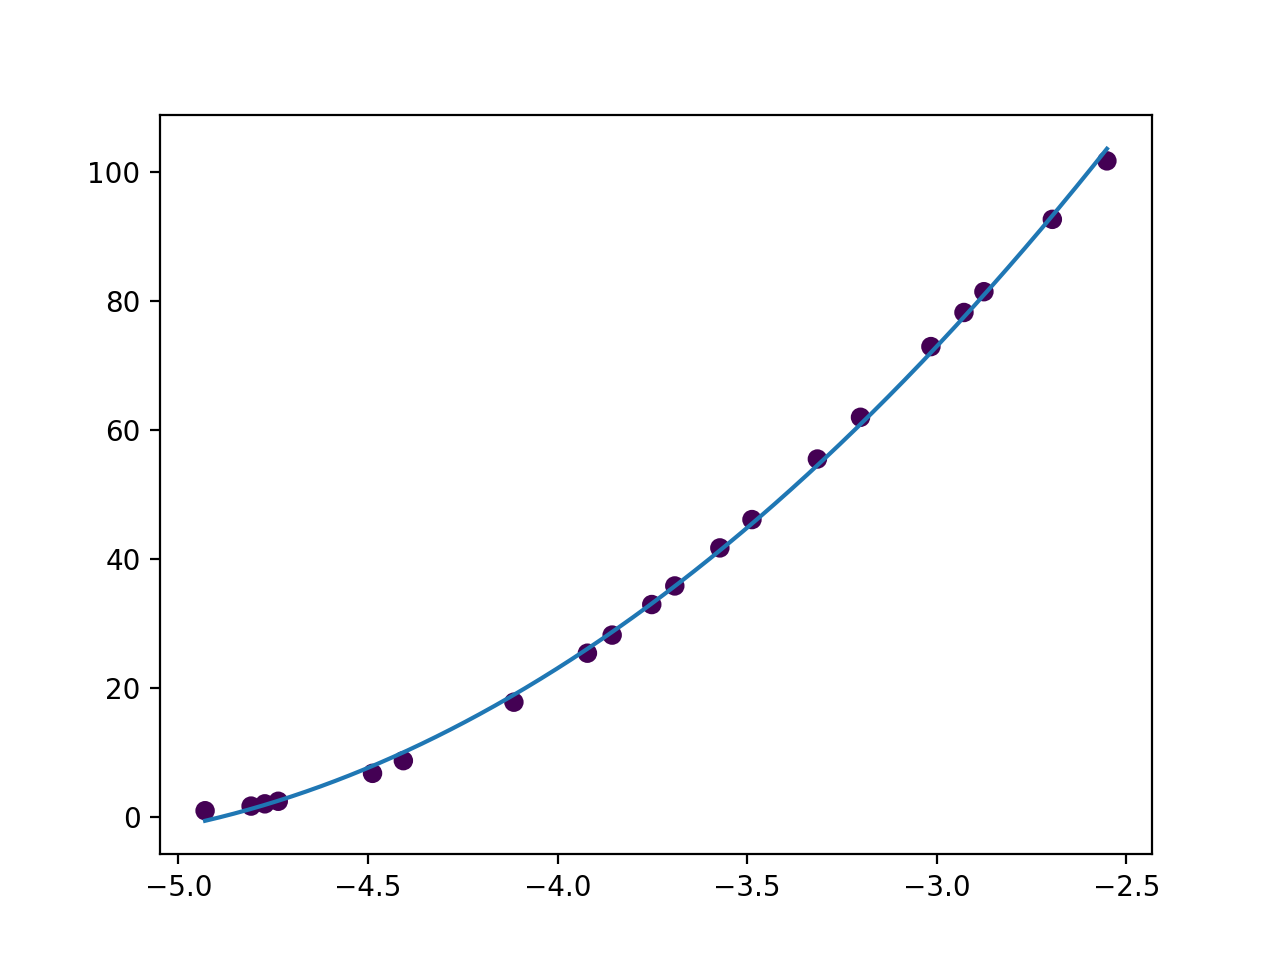
\includegraphics[width = 0.45\textwidth]{images/basic_3_quadratic.png}\label{fig:basic_3_quadratic.csv}}
    \hfill
    \subfloat[Cubic fit]{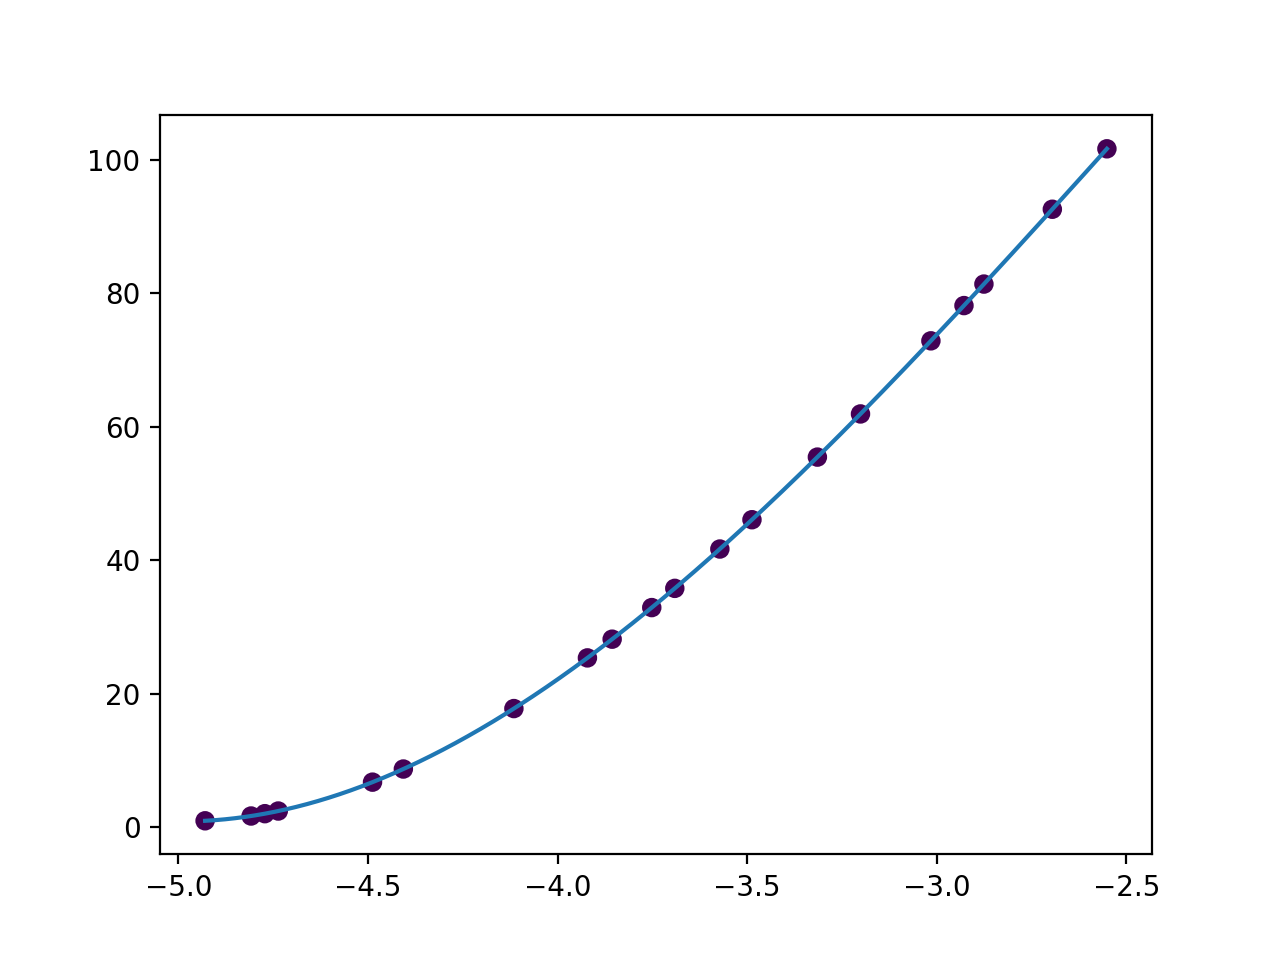
\includegraphics[width = 0.45\textwidth]{images/basic_3.png}\label{fig:basic_3_cubic.csv}}
    \caption{Two fits for `\texttt{basic\_3.csv}'}
    \label{fig:basic_3.csv}
\end{figure}

To confirm this visually, I used the `\texttt{basic\_*.csv}' files
as they have a negligable amount of noise.
I produced fits using several different polynomials.
An example of this is shown in Figure \ref{fig:basic_3.csv}.
The quadratic fit shown in Figure \ref{fig:basic_3_quadratic.csv}
is clearly not as good a fit as the cubic fit shown in Figure \ref{fig:basic_3_cubic.csv}.

\section{Choice of unknown function}

Using my `\texttt{display.py}' program to visualise the
signals, I produced a list of potential `unknown functions'
that could represent the underlying signal of line segments
based on their shapes:
$\vb{w}_{1}sin(x) + \vb{w}_{2}$,
$\vb{w}_{1}cos(x) + \vb{w}_{2}$,
$\vb{w}_{1}tan(x) + \vb{w}_{2}$ and
$\vb{w}_{1}e^{x} + \vb{w}_{2}$.
I then created a program, `\texttt{unknown.py}', that
calculated the cross-validation error for each of the
nonlinear line segments previously identified when
trained using each of the potential unknown functions.
A table displayed the cross-validation errors---similar 
to that used to determine the polynomial degree.
Having analysed the cross-validation errors, it was clear
that all nonlinear signals that were likely not
a cubic polynomial had their minimum cross-validation
error when trained to fit the function
$\vb{w}_{1}sin(x) + \vb{w}_{2}$.
This consistent minimum cross-validation error indicated
that the `unknown function' used to generate the unknown
signals is of the form $\vb{w}_{1}sin(x) + \vb{w}_{2}$.

\begin{figure}[htbp]
    \centering
    \subfloat[Cosine fit]{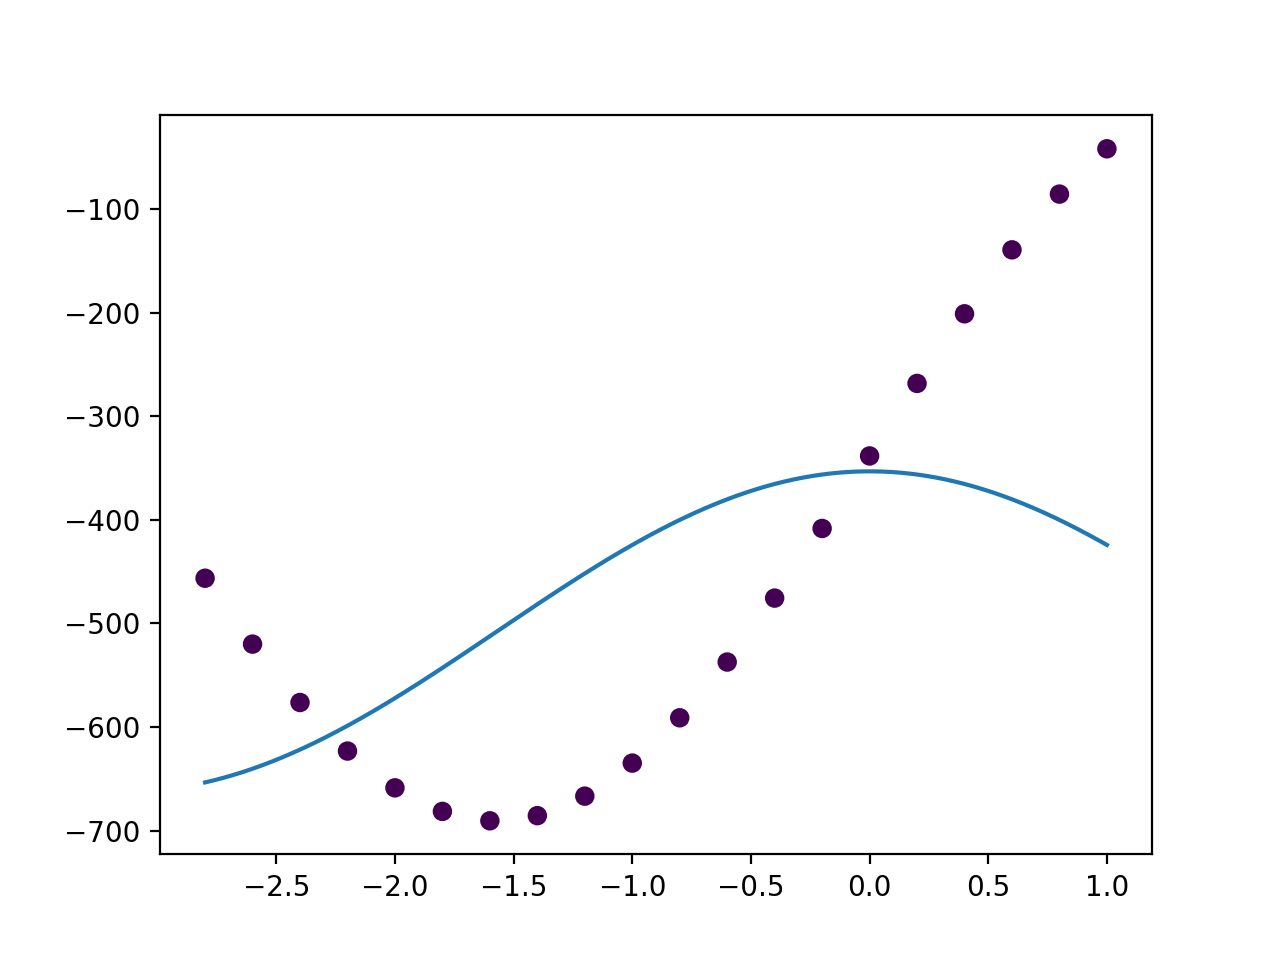
\includegraphics[width = 0.45\textwidth]{images/basic_5_cosine.png}\label{fig:basic_5_cosine.csv}}
    \hfill
    \subfloat[Sine fit]{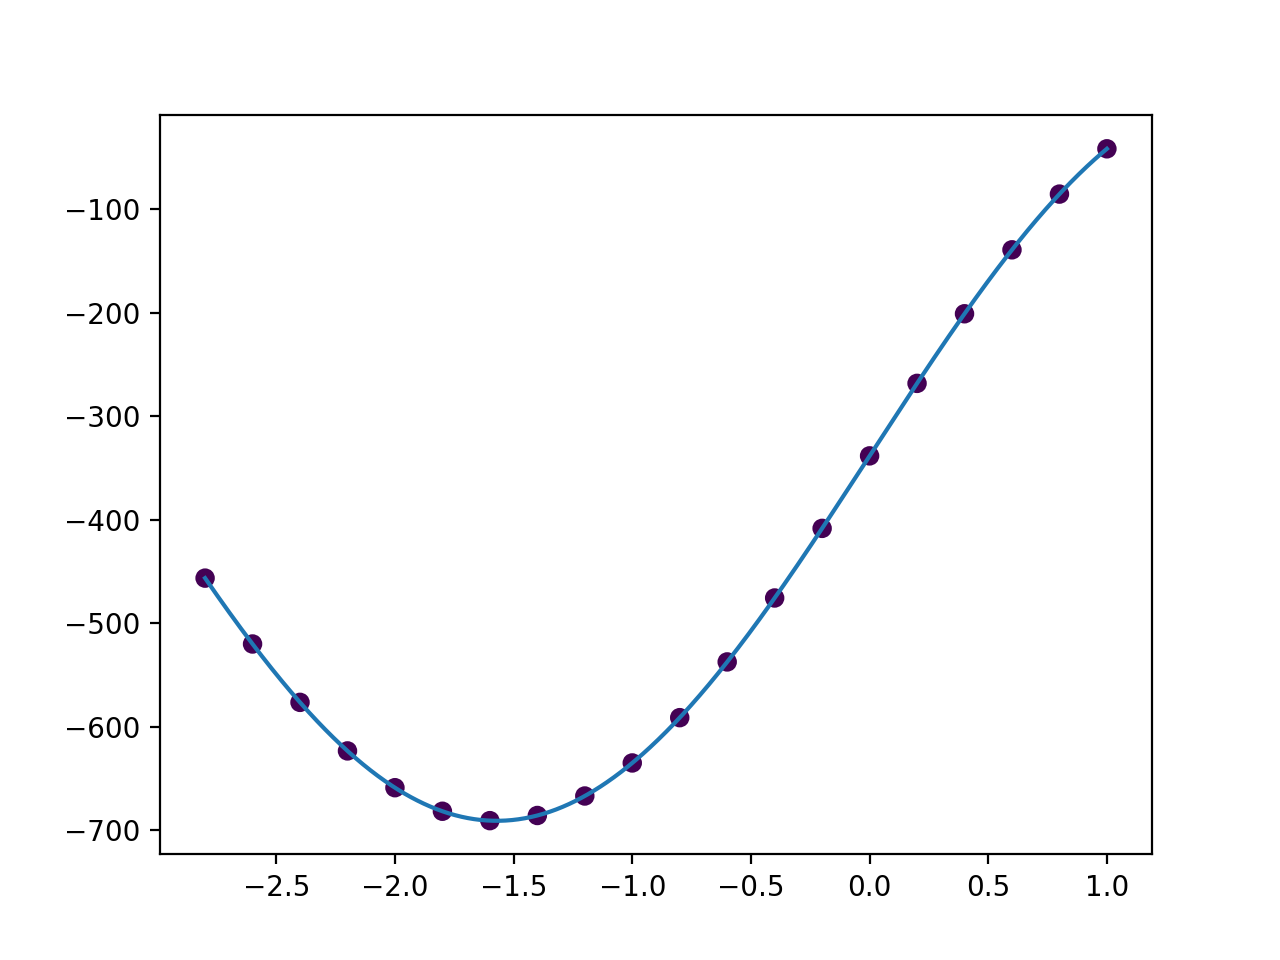
\includegraphics[width = 0.45\textwidth]{images/basic_5.png}\label{fig:basic_5_sine.csv}}
    \caption{Two fits for `\texttt{basic\_3.csv}'}
    \label{fig:basic_5.csv}
\end{figure}

`\texttt{basic\_5.csv}' was the only one of the
`\texttt{basic\_*.csv}' files to not fit linear and
cubic functions exactly, which strongly indicated that it was generated from
the unknown function. 
Thus, due to its negligable amount of noise,
I used it to verify that the unknown function was
$\vb{w}_{1}sin(x) + \vb{w}_{2}$.
To do so, I produced a fit for each of the potential
unknown functions.
An example of this is shown in Figure \ref{fig:basic_5.csv}.
The cosine fit shown in Figure \ref{fig:basic_5_cosine.csv}
is a far worse fit than the sine fit shown in Figure
\ref{fig:basic_5_sine.csv}, which fits almost perfectly.

\section{Model selection}

\begin{figure}[htbp]
    \centering
    \subfloat[Cubic fit]{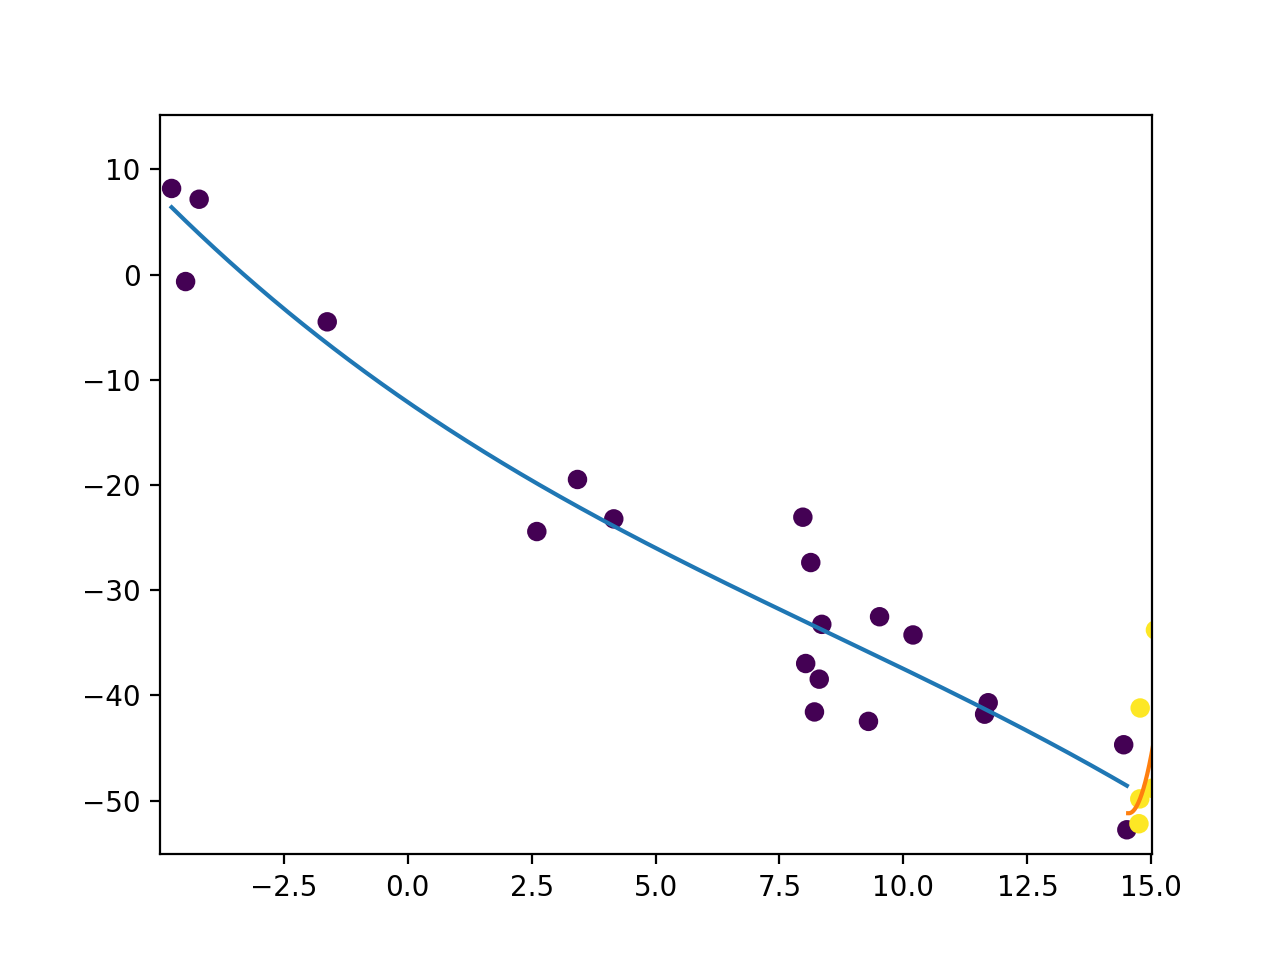
\includegraphics[width = 0.45\textwidth]{images/noise_2_0_polynomial.png}\label{fig:noise_2_polynomial.csv}}
    \hfill
    \subfloat[Linear fit]{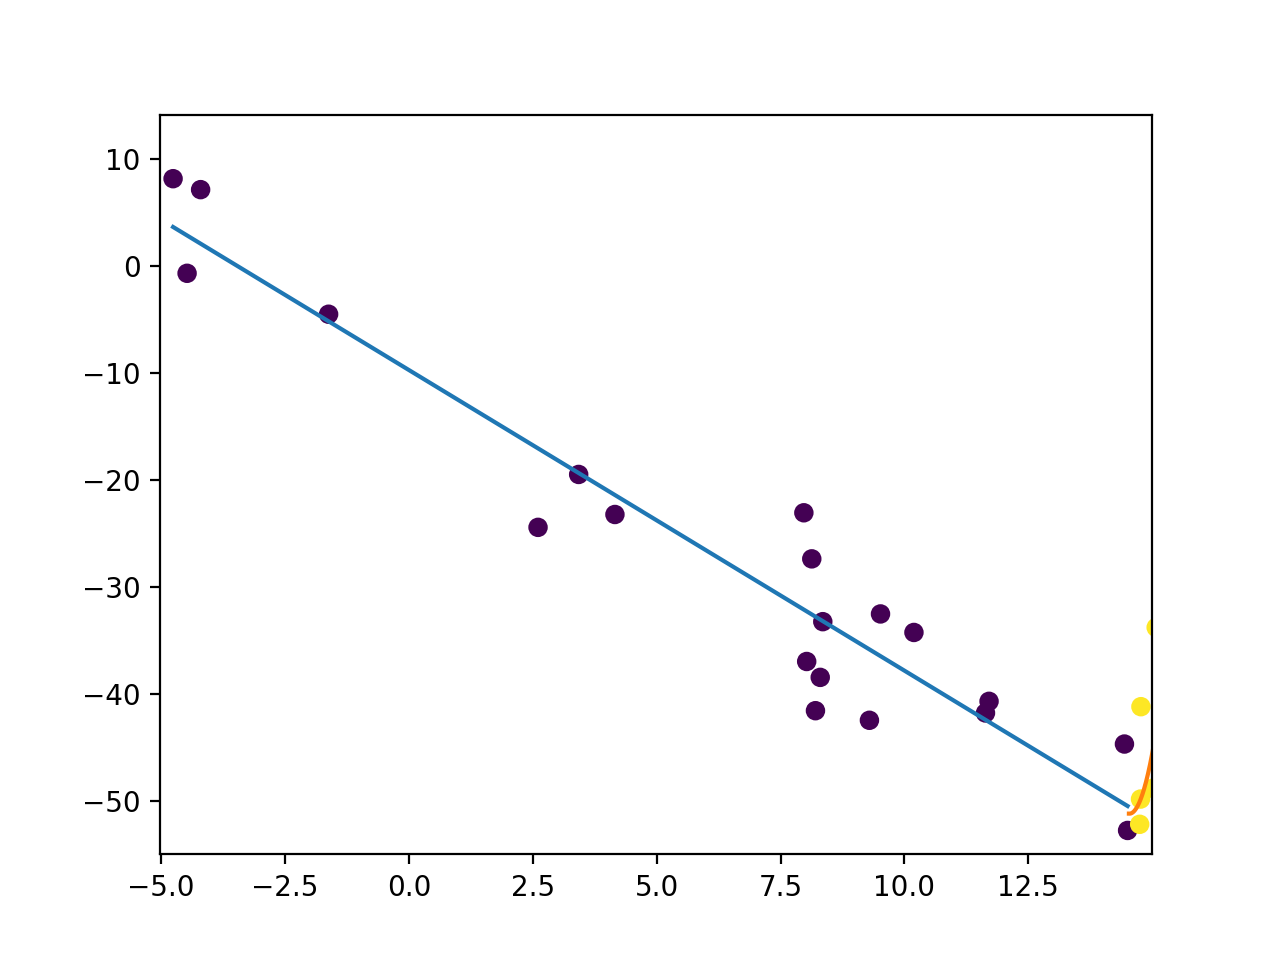
\includegraphics[width = 0.45\textwidth]{images/noise_2_0_linear.png}\label{fig:noise_2_linear.csv}}
    \caption{Two fits for the first line segment in `\texttt{noise\_2.csv}'}
    \label{fig:noise_2.csv}
\end{figure}

Overfitting occurs when a machine learning algorithm
produces a model that has learnt the noise in the data
as if it represents the structure of the underlying
model \cite{MSMI}.
In the case of linear regression, overfitting is most
likely to occur by producing a model with too complex a function
type, such that it would fail to predict future observations.
Figure \ref{fig:noise_2.csv} shows an example of this. 
Figure \ref{fig:noise_2_polynomial.csv} shows a cubic fit that is too complex a 
function type for the data points.
It would not predict future $y$-values for a set of 
given $x$-values as successfully as the linear fit shown in Figure \ref{fig:noise_2_linear.csv}

My original implementation used the holdout method
to detect overfitting, and determine the best model for a given line segment.
However, despite experimenting with different
sized training and validation sets, my program was consistently
giving misleading results---both overfitting and underfitting.
This is because the holdout method involved only a single run,
and so was dependent on how the datapoints were randomly
split into training and validation sets.
Due to the limited number of data points in each line segment,
this resulted in the program often producing wildly different results.
On the other hand, as the holdout method only involved a single run, it was fast.

Despite the speed of the holdout method, I wanted my increase the accuracy
of my program.
To do so, I implemented $k$-fold cross-validation.
In particular, I opted to use leave-one-out cross-validation.
Leave-one-out cross-validation is 
an extreme case of $k$-fold cross validation
such that $k = n$, where
$n$ is the number of data points (in this case, 20).
Leave-one-out cross-validation involves using each of
the 20 data points in a given line segment exactly once as validation data for a model
trained using the other 19 data points. 
The cross-validation error for each function type is calculated
as follows \cite{Stanford}:
\[
    CV_{(n)} = \frac{1}{n} \sum_{i = 1}^{n} (y_{i} - \hat{y}^{(-i)})^{2}
\]
where
$n$ is the number of data points in a line segment (i.e. 20),
$y_{i}$ is the actual $y$-value for the $i$-th data point,
and $\hat{y}^{(-i)}$ is the predicted $y$-value for the $i$-th
data point when trained without using the $i$-th sample.

As a result of having to produce $n$ different models,
leave-one-out cross-validation can be computationally expensive.
However, owing to the limited sample size of each line segment,
I believe it to be an appropriate technique to use in this case---on
most modern computers, it takes very little time
to produce twenty different models.
Additionally, the result is completely deterministic, as it does not depend
on a random seed, and so is far less unstable than the holdout method.
Leave-one-out cross-validation is also a less biased technique
than $k$-fold cross-validation with values of $k < n$.

The function type with the lowest cross-validation error
is then selected for each line segment,
and the weights $\vb{\hat{w}}$ are determined by training on all
data points for that segment.

\section{Optimisations and improvements}

To begin with,
computing the matrix inverse using the \texttt{np.linalg.inv}
method is computationally expensive and unnecessary.
Instead, given $\vb{X}$ and $\vb{y}$, the maximum likelihood
estimation of $\vb{w}$ could be directly computed as follows:
\texttt{np.linalg.solve(X.T @ X, X.T @ y)}.
Computing $\vb{\hat{w}}$ directly would be faster, as \texttt{np.linalg.inv}
computes the inverse of a matrix $\vb{A}$ by solving for $\vb{A}^{-1}$
in $\vb{AA^{-1} = I}$ \cite{StackOverflow}.
Thus, there would be a performance benefit by solving for
$\vb{\hat{w}}$ in
$\vb{X}^{T} \vb{X} \vb{\hat{w}} = \vb{X}^{T} \vb{y}$ directly.

Another computationally expensive operation in my
algorithm is that used to calculate the cross-validation error 
using leave-one-out cross-validation.
The method currently involves
fitting the model and calculating the sum squared error
$n$ times. 
Instead, there exists a faster method I could have
adopted that involves calculating the leverage.
Despite this, I opted not to include this method 
because my program, as it currently stands, can be 
easily adapted to use $k$-fold cross-validation for 
any value of $k$ that is a factor of the number of points in each line segment---changing
the constant `\texttt{K}' in the code achieves this.

\section{Testing}

I created a file, `\texttt{test.py}', that uses the
\texttt{unittest} framework to test each of the methods
in `\texttt{lsr.py}'.

\clearpage
\begin{thebibliography}{9}

    \bibitem{MSMI}
    Burnham, K. P. and Anderson, D. R. (2002)
    \textit{Model Selection and Multimodel Inference}.
    2nd ed. Springer-Verlag.

    \bibitem{Stanford}
    Taylor, J. (2020)
    \textit{Leave one out cross-validation (LOOCV) --- STATS 202}
    https://web.stanford.edu/class/stats202/notes/Resampling/LOOCV.html

    \bibitem{StackOverflow}
    Muldal, A. (2017)
    \textit{Why does numpy.linalg.solve() offer more precise matrix inversions than numpy.linalg.inv()?}
    https://stackoverflow.com/a/31257909/8540479



\end{thebibliography}
    

\end{document}
